\section{Desarrollo Configuración}


A continuación se presenta el procedimiento que se debe llevar a cabo para configurar la maquina que actúa como maestro, a la cual se le realiza la replica. Luego se dará paso a la configuración de la maquina esclavo. Este proceso se realiza por medio de la herramienta PuTTY, que nos permite tener conexión al S.O centos 7 desde Windows.\\

\subsection*{Configuración de la maquina "Maestro"}
Inicialmente se realiza la conexión a la maquina que actúa como maestro por medio del usuario root y la clave correspondiente, luego se ingresa al archivo hosts, como se muestran en la Figura \ref{fig:1}.

\begin{figure}[H]
\centering
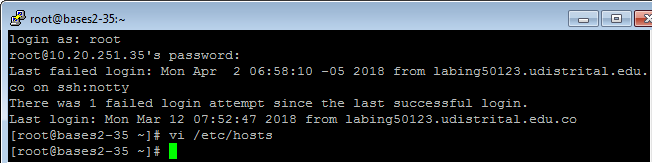
\includegraphics[width=\columnwidth]{eRelatedWorks/src/1}
\caption{Ingreso al archivo hosts. }\label{fig:1}
\end{figure}

Tal como se presenta en la Figura \ref{fig:2}, en el archivo hosts se agrega una linea con la dirección IP y el dominio de la maquina que actúa como esclavo, en este caso IP 10.20.251.28 y dominio bases2-28.udistrital.edu.co.

\begin{figure}[H]
\centering
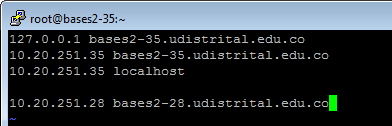
\includegraphics[width=\columnwidth]{eRelatedWorks/src/2}
\caption{Modificación al archivo hosts. }\label{fig:2}
\end{figure}

Antes de iniciar el proceso de configuración del maestro es importante realizar un backup del archivo postgresql.conf, esta copia ante futuros errores es de gran utilidad. En la Figura \ref{fig:3} se observa como crear la copia con el comando cp y luego con el comando ls se comprueba si fue creada. Es importante aclarar que dicho proceso se realiza desde el directorio data, que pertenece al usuario postgres. 

\begin{figure}[H]
\centering
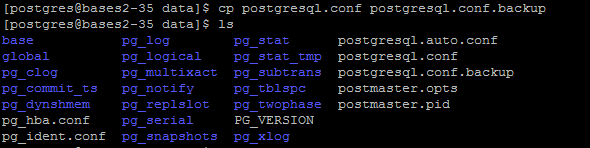
\includegraphics[width=\columnwidth]{eRelatedWorks/src/3}
\caption{Backup a archivo postgresql.conf. }\label{fig:3}
\end{figure}

Al estar activo con el usuario postgres se crea el usuario de replicación repuser y se asgina una contraseña como se indica en la Figura \ref{fig:4}.

\begin{figure}[H]
\centering
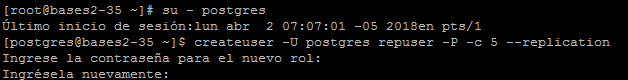
\includegraphics[width=\columnwidth]{eRelatedWorks/src/4}
\caption{Creación del usuario de replicación. }\label{fig:4}
\end{figure}

Se ingresa al archivo pg\_hba.conf con la linea de código que se muestra en la Figura \ref{fig:5}.

\begin{figure}[H]
\centering
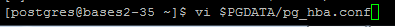
\includegraphics[width=\columnwidth]{eRelatedWorks/src/5}
\caption{Ingreso al archivo pg\_hba.conf. }\label{fig:5}
\end{figure}

En el archivo pg\_hba.conf se agrega la ultima linea que se muestra en la Figura \ref{fig:5}, estos son los datos referentes a la maquina esclavo, entre estos datos se encuentra el nombre del usuario creado en la Figura \ref{fig:4} y la IP de la maquina esclavo. Con se permite al servidor esclavo de IP 10.20.251.28, conectarse al servidor maestro con permiso de replicación.

\begin{figure}[H]
\centering
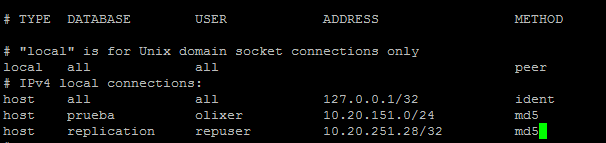
\includegraphics[width=\columnwidth]{eRelatedWorks/src/6}
\caption{Modificación del archivo pg\_hba.conf. }\label{fig:6}
\end{figure}

Se ingresa al archivo postgresql.conf con la linea de código que se muestra en la Figura \ref{fig:7}.


\begin{figure}[H]
\centering
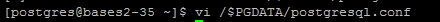
\includegraphics[width=\columnwidth]{eRelatedWorks/src/7}
\caption{Ingreso al archivo postgresql.conf. }\label{fig:7}
\end{figure}

A continuación se presenta las diferentes modificaciones que se deben realizar en el archivo postgresql.conf. La primera es activar la opción de "wal\_level", la cual define cuanta información se grabará en los archivos WAL generados. Se le asigna un estado de hot\_standby como se refleja en la Figura \ref{fig:8}.
\begin{figure}[H]
\centering
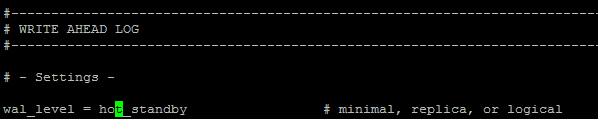
\includegraphics[width=\columnwidth]{eRelatedWorks/src/8}
\caption{Opción wal\_level. }\label{fig:8}
\end{figure}

Como se muestra en la Figura \ref{fig:9} se activa la opción archive\_mode y se le asigna un estado on. Dicha opción define la habilitación de archivos WAL en el servidor maestro.

\begin{figure}[H]
\centering
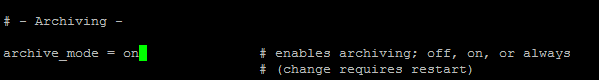
\includegraphics[width=\columnwidth]{eRelatedWorks/src/9}
\caption{Opción archive\_mode.  }\label{fig:9}
\end{figure}

En la Figura \ref{fig:10} se activa la opción archive\_command, la cual define la copia de registros WAL a archivar en el servidor maestro y transferirlos al servidor esclavo. Es importante aclarar que esta linea de código para que este activa no debe tener el símbolo \# al inicio. 

\begin{figure}[H]
\centering
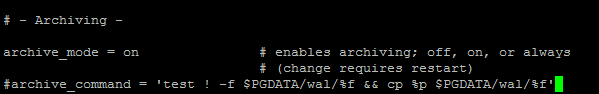
\includegraphics[width=\columnwidth]{eRelatedWorks/src/10}
\caption{Opción archive\_command.}\label{fig:10}
\end{figure}

Se activa la opción max\_wal\_senders la cual define las conexiones concurrentes o cuantos servidores de Standby se van a conectar al servidor maestro. En el presente caso el numero de servidores es de 3 como se muestra en la Figura \ref{fig:11}. Luego de esto se procede a guardar los cambios efectuados. 

\begin{figure}[H]
\centering
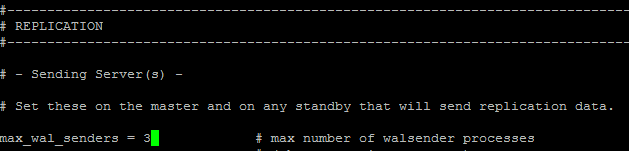
\includegraphics[width=\columnwidth]{eRelatedWorks/src/11}
\caption{Opción max\_wal\_senders. }\label{fig:11}
\end{figure}

Después de guardar los cambios efectuados en el archivo postgresql.conf, se procede a reiniciar  el servidor con el comando pg\_ctl restart como se muestra en la Figura \ref{fig:12}. Después de un reinicio exitoso, ejecutamos el comando psql, si se ingresa al usuaio postgres esto  nos afirma que momentáneamente los cambios realizados se hicieron correctamente. 

\begin{figure}[H]
\centering
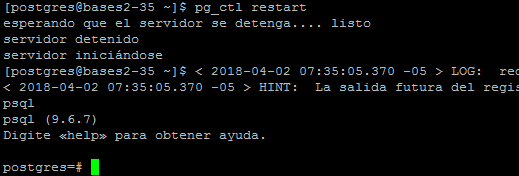
\includegraphics[width=\columnwidth]{eRelatedWorks/src/12}
\caption{Reinicio del servidor}\label{fig:12}
\end{figure}

\subsection*{Configuración de la maquina "Esclavo"}

En el siguiente desarrollo del documento se presentaran los respectivos screenshot de la configuración de la máquina "esclavo" de este modo queda complementada la replicación y su pasan a realizar pruebas del correcto funcionamiento de la misma.

\begin{figure}[H]
\centering
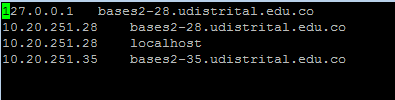
\includegraphics[width=\columnwidth]{eRelatedWorks/src/Captura1}
\caption{Configuración Esclavo 1. }\label{figC:1}
\end{figure}

La primera configuración a realizar dentro de la máquina esclava, es relacionar la dirección ip y host de la máquina maestro, siendo la máquina maestro \textbf{10.20.251.35} en la figura \ref{figC:1} a esta configuración se accede mediante el archivo que se visualiza en la figura \ref{figC:2}

\begin{figure}[H]
\centering
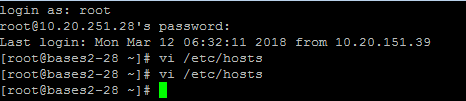
\includegraphics[width=\columnwidth]{eRelatedWorks/src/Captura2}
\caption{Configuración Esclavo 2. }\label{figC:2}
\end{figure}

\begin{figure}[H]
\centering
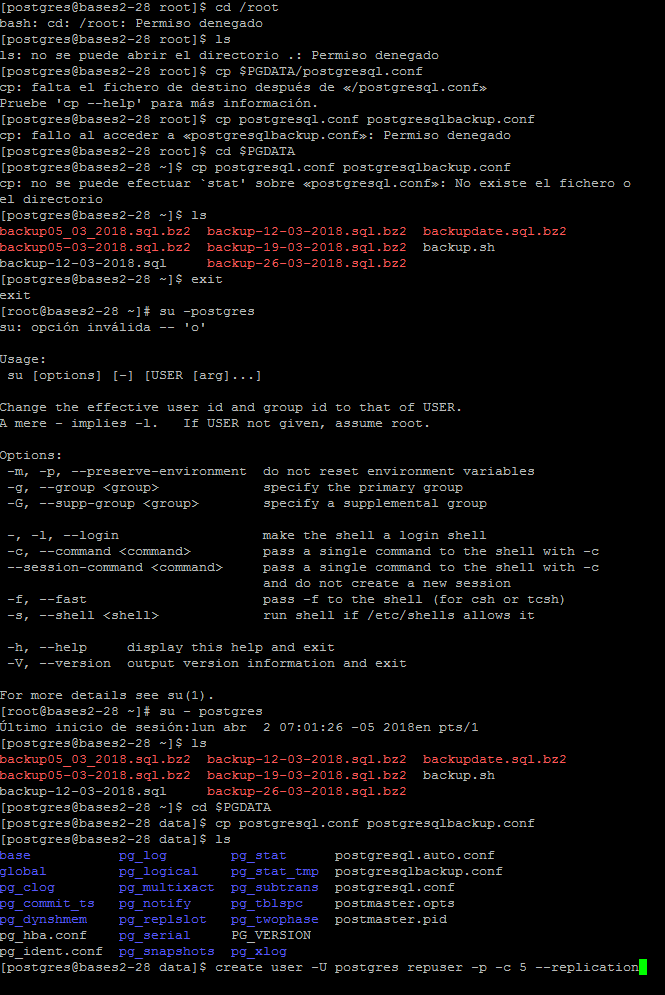
\includegraphics[width=\columnwidth]{eRelatedWorks/src/Captura3}
\caption{Configuración Esclavo 3. }\label{figC:3}
\end{figure}

En la figura \ref{figC:3} se conecta al servidor de la base de datos postrgres y se realiza la creación del usuario encargado de recibir la replicación por parte del maestro, ésto posible con la bandera \textbf{\textit{--replication}}, dicha creacion del usuario solicitara la contraseña para el rol esto se visualiza en la figura \ref{figC:4}, luego de todo ellos se crea la carpeta wal en \$PGDATA

\begin{figure}[H]
\centering
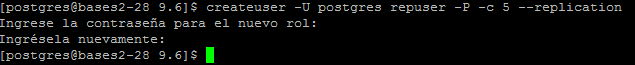
\includegraphics[width=\columnwidth]{eRelatedWorks/src/Captura4}
\caption{Configuración Esclavo 4. }\label{figC:4}
\end{figure}

\begin{figure}[H]
\centering
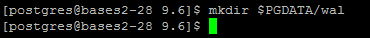
\includegraphics[width=\columnwidth]{eRelatedWorks/src/Captura5}
\caption{Configuración Esclavo 5. }\label{figC:5}
\end{figure}

Hecho esos pasos de creación de usuarios dentro de postgres se debe asociar dentro del archivo de configuración, allí se relaciona la base de datos, el usuario, la dirección y el método \textbf{\textit{md5}} esto se refleja en la figura \ref{figC:6}, esto se logra accediendo al fichero visualizado en la figura \ref{figC:7}, en dicha configuración debe accederse a la sección relacionada y agregar los valores que fueron creados en pasos anteriores.

\begin{figure}[H]
\centering
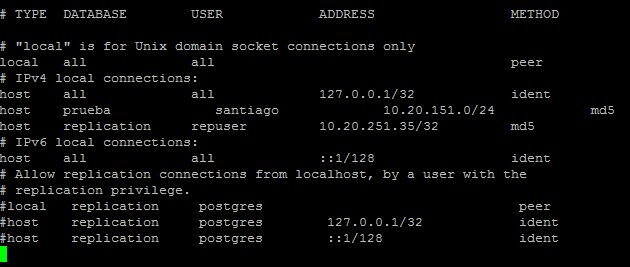
\includegraphics[width=\columnwidth]{eRelatedWorks/src/Captura6}
\caption{Configuración Esclavo 6. }\label{figC:6}
\end{figure}

\begin{figure}[H]
\centering
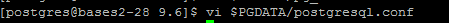
\includegraphics[width=\columnwidth]{eRelatedWorks/src/Captura7}
\caption{Configuración Esclavo 7. }\label{figC:7}
\end{figure}

Otro aspecto importante a revisar dentro de este archivo es la configuracion del atributo \textit{wal\_level} y debe ser asignado en valor de \textit{hot\_standy} es el término utilizado para describir la capacidad de conectarse al servidor y ejecutar consultas de solo lectura mientras el servidor está en recuperación de archivos o modo de espera. 

Esto es útil tanto para fines de replicación como para restaurar una copia de seguridad a un estado deseado con gran precisión. El término Hot\_Standby también se refiere a la capacidad del servidor para pasar de la recuperación a la operación normal mientras los usuarios continúan ejecutando consultas y / o mantienen sus conexiones abiertas.

\begin{figure}[H]
\centering
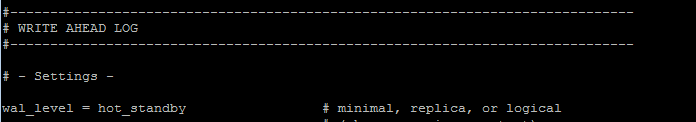
\includegraphics[width=\columnwidth]{eRelatedWorks/src/Captura8}
\caption{Configuración Esclavo 8. }\label{figC:8}
\end{figure}

En la figura \ref{figC:9} se muestra el estado en el cual debe quedar la configuracion de \textit{arhive\_mode} 

\begin{figure}[H]
\centering
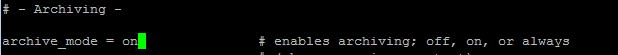
\includegraphics[width=\columnwidth]{eRelatedWorks/src/Captura9}
\caption{Configuración Esclavo 9. }\label{figC:9}
\end{figure}

Otras configuraciónes figuran en \ref{figC:10} y \ref{figC:11} en donde se configura max\_wal\_senders que especifica la cantidad máxima de conexiones concurrentes desde servidores en espera o clientes de copia de seguridad de transmisión por secuencias

\begin{figure}[H]
\centering
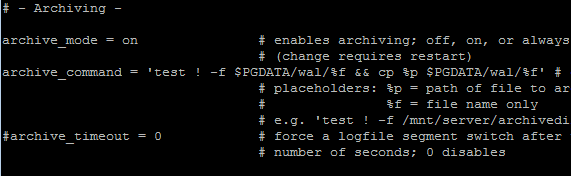
\includegraphics[width=\columnwidth]{eRelatedWorks/src/Captura10}
\caption{Configuración Esclavo 10. }\label{figC:10}
\end{figure}


\begin{figure}[H]
\centering
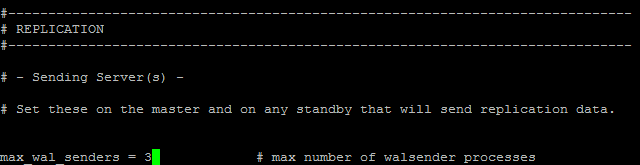
\includegraphics[width=\columnwidth]{eRelatedWorks/src/Captura11}
\caption{Configuración Esclavo 11. }\label{figC:11}
\end{figure}

\begin{figure}[H]
\centering
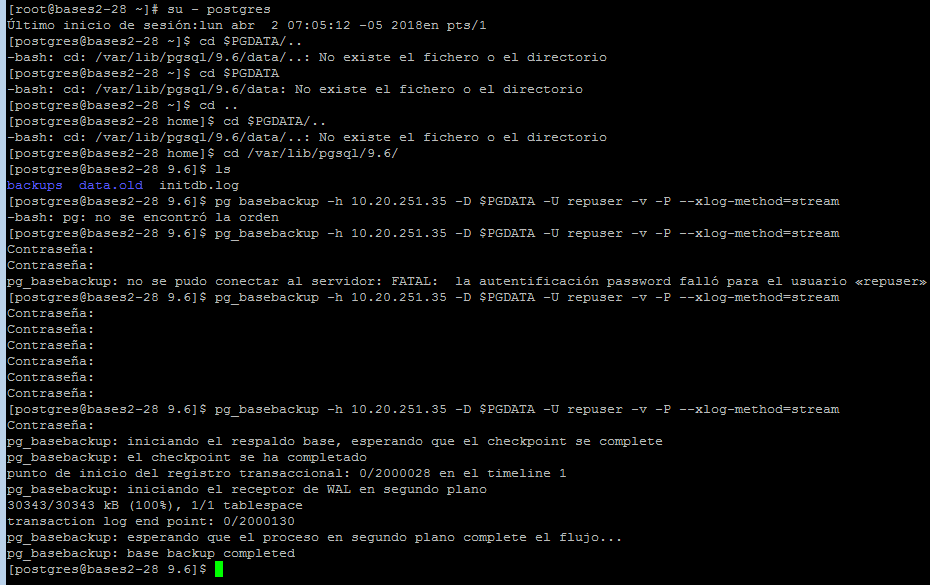
\includegraphics[width=\columnwidth]{eRelatedWorks/src/Captura12}
\caption{Configuración Esclavo 12. }\label{figC:12}
\end{figure}

En esta figura final se busca mostrar todo el proceso donde de conexión con el usuario creado en pasos anteriores y donde se genera el respaldo de la base.

